\section{Experiments}

We connect our theory to pratical problems of interest.
(i) We validate the single-task based metric on text and image classification tasks.
We show that for both datasets, single-task learning results can help predict positive or negative transfer in multi-task learning.
(ii) We show that our proposed incremental training schedule improves the training efficiency of multi-task learning for predicting a particular target task.
%Third, we measure the data efficiency ratio of multi-task learning on six sentiment analysis tasks.
(iii) We validate our theoretical results in Section \ref{sec_insight} on text classification tasks.

\begin{table}[!b]
\begin{minipage}[t]{.40\textwidth}
	\vspace{-0.1in}
	\centering
	\begin{tabular}{c c c}
		\toprule
		\multirow{2}{*}{{\bf Models}} & \multicolumn{2}{c}{\begin{minipage}{1.1in}\begin{center}
		Sentiment\\ analysis\end{center}\end{minipage}} \\
		\cmidrule(lr){2-3}
		& {\bf MTL} & {\bf IncTrain} \\
		\midrule
		{\bf MLP}  & 100\% & \textbf{xx\%} \\
		{\bf LSTM} & \textbf{36\%} & xx\% \\
		\bottomrule
		\end{tabular}
	\vspace{0.1in}
	\captionof{table}{Measuring the data efficiency ratio of muli-task learning.}
	\label{tab:taskonomy}
\end{minipage}%
\quad
\begin{minipage}[t]{.58\textwidth}
	\vspace{-0.1in}
	\centering
  \begin{tabular}{c c c c c}
	\toprule
		\multirow{2}{*}{{\bf Threshold}}  & \multicolumn{2}{c}{{\bf Sentiment
		analysis}} & \multicolumn{2}{c}{{\bf ChestX-ray14}} \\
		& Precision &  Recall & Precision &  Recall \\
		\cmidrule(lr){1-1} \cmidrule(lr){2-3} \cmidrule(lr){4-5}
		0.0 & 0.596 & 1.000 & 0.593 & 1.000 \\
		0.1 & \textbf{0.756} & \textbf{0.388} & \textbf{0.738} & \textbf{0.462} \\
		0.2 & 0.919 & 0.065 & 0.875 & 0.044 \\
		% 0.3 & 1.000 & 0.004 &     - &     - \\
	\bottomrule
	\end{tabular}
	\vspace{0.1in}
	\captionof{table}{Single-task learning results can help predict postive or negative transfer in multi-task learning.}
	\label{tab:mtl_better_than_stl}
\end{minipage}
\end{table}

\subsection{Experimental Setup}

We consider a text classification task and an image classification task as follows.

{\it Sentiment Analysis:} This dataset includes six tasks: movie review sentiment (MR), sentence subjectivity (SUBJ), customer reviews polarity (CR), question type (TREC), opinion polarity (MPQA), and the Stanford sentiment treebank (SST) tasks.
{For each task, the goal is to categorize sentiment opinions expressed in the text.
We use an embedding layer with GloVe embeddings
followed by an LSTM or MLP layer proposed by~\cite{lei2018simple}.
}
%multi-layer perceptron (MLP), LSTM, CNN on all tasks
%We use this task to verify our theoretical results on model capacity and task covariance in real world.

{\it ChestX-ray14:} This dataset contains 112,120 frontal-view X-ray images and each image has up to 14 diseases.
This is a 14-task multi-label image classification problem.
%We treat each label as one task a binary classification problem and formulate it as a 14-task multi-task learning problem.
%This dataset is curated where the labels
%We use the CheXNet model from~\cite{chexnet}, which is a 121-layer convolutional neural network on all tasks.


%\textbf{The training procedure and baseline.}
For all models, we share the main module across all tasks and assign a separate regression or classification layer on top of the shared module for each tasks.
The baseline training schedule for MTL is the round-robin training schedule.
%We compare our incremental training schedule of Algorithm \ref{alg_inc_train} to the round-robin training schedule.
We measure the test accuracy of predicting a target task.


\subsection{Experimental Results}

Our first result is to show that our proposed incremental training schedule (Algorithm \ref{alg_inc_train}) can help mitigate negative transfer for predicting a particular target task.
Our insight is that since adding more samples from the source task does not always improve performance, we can improve efficiency by adding the source samples \textit{incrementally} during training.
Over six randomly selected task pairs from the sentiment analysis dataset, we find that Algorithm \ref{alg_inc_train} requires only $45\%$ of the computational cost to achieve the same performance on the target task, compared to the multi-task learning baseline.

%\textbf{Improving transfer learning training efficiency.}
%We show that Algorithm \ref{alg_inc_train} also applies to transfer learning settings.
%Compared to fine-tuning the source model on the target task, we show that our proposed method reduces the computional cost by \alert{$xx\%$}, without sacrificing accuracy.

We measure the data efficiency ratio on the sentiment analysis tasks.
In Table \ref{tab:taskonomy}, we find that by performing multi-task learning, only $39\%$ ({\cor or $36\%$?}) of the labeled data is needed to achieve comparable performance to single-task learning over all six tasks on LSTM.
The data efficiency ratio of using MLP is $100\%$ because the average performance of MTL is worse than the average of STL.
We further show that applying incremental training helps reduce the data efficiency ratio to \alert{$xx\%$}.
%If TREC is not included, we see that only $25\%$ of the labeled data is needed.


\begin{figure}[!t]
	\centering
	\begin{subfigure}[b]{0.33\textwidth}
		\centering
		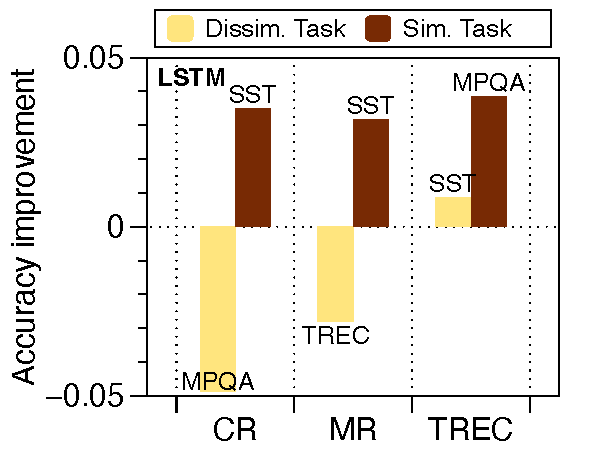
\includegraphics[width=0.975\textwidth]{figures/task_sim_norm_lstm.pdf}
		\caption{Task similarity}
		\label{fig_ab_sim}
	\end{subfigure}%
	\begin{subfigure}[b]{0.33\textwidth}
		\centering
		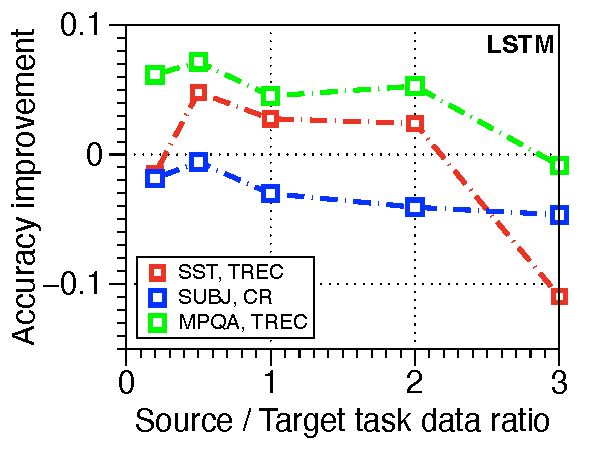
\includegraphics[width=0.975\textwidth]{figures/ratio_norm_3_pairs_lstm.pdf}
		\caption{Data size}
		\label{fig_ab_data}
	\end{subfigure}
	\begin{subfigure}[b]{0.33\textwidth}
		\centering
		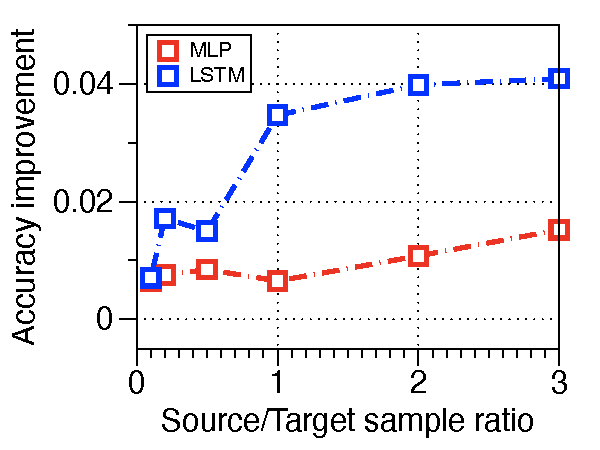
\includegraphics[width=0.975\textwidth]{figures/ratio_alignment_norm_diff_all.pdf}
		\caption{Covariate shift}
		\label{fig_ab_cov}
	\end{subfigure}
	\caption{Validating the three results of Section \ref{sec_insight} on sentiment analysis tasks. (a) Adding a semantically similar source task in MTL performs better than adding a dissimilar task.
	(b) As source/target sample ratio increases, we observe a transition from positive to negative transfer (red curve).
	(c) As source/target sample ratio increases, the performance gain of aligning task covariances \cite{WZR20} compared to MTL increases for LSTM and MLP.}
	\label{fig_ablation}
	\vspace{-0.15in}
\end{figure}


\subsection{Ablation Studies}

A common challenge in the study of multi-task learning is that the results can be hard to understand.
It is difficult to predict when MTL performs well without running extensive trials.
Our insight here is that we can use STL results to help understand MTL results.
We validate the single-task based metric proposed in Section \ref{sec_similarity} for predicting positive or negative transfer in MTL.
Table \ref{tab:mtl_better_than_stl} shows the result on both the sentiment analysis and the ChestX-ray14 tasks.
We find that using a threshold of $\tau = 0.1$, the STL results correctly predict positive or negative transfer with $75.6\%$ accuracy and $38.8\%$ recall among $30$ times $5$ (random seeds) task pairs!
We observe similar results for $91$ task pairs from the ChestX-ray14 dataset.
The results show that STL results are indicative of MTL results.


Finally, we validate our theoretical results in Section \ref{sec_insight} on the sentiment analysis tasks.
In Figure \ref{fig_ablation}, we show that MTL performance is affected by
(a) decreased task similarity;
(b) increased source/target sample ratio;
(c) covariate shift under increased source sample size.
For the last result, specifically we show that the alignment procedure proposed in \cite{WZR20} becomes more helpful when the sample ratio is large.
The experimental procedure is left to Appendix \ref{app_it}.


